MongoDB is a schema-less document-oriented database developed by MongoDB Inc. with the support of Open Source community. 
\subsubsection{Data design} 
\paragraph{Document}
	A document is abstract and storable unit in MongoDB. It is the data structure expressed in the form of JSON and is stored in BSON, a binary variant of JSON that supports additional data types like ObjectId, timestamp, datetime etc. All the accessible data including database records, query selectors, index specifications, server configurations etc. are represented as documents. An example  MongoDB document is given in Figure~\ref{sample-mongodb-document}.
Every document is referenced with a unique key. A document is retrieved either by the key or any other attribute of the document. Collection in MongoDB is a group of documents and it is stored in a database. It is more convenient to group similar structured documents in a collection but not mandatory. MongoDB has two principles that allow the users to represent the relationships between the documents: \textit{references} and \textit{embedded} documents~\citep{mongodb:org}. 
\begin{description}
\item[Embedded]\label{mongo:embedded} \hfill \\
    In Embedded document, data is nested. The documents are structured as sub-document in the form of Arrays or Objects~\citep{nosql/comparision}. 
    \item[References] \hfill \\
    Unlike RDBMS, MongoDB has no support for joins, therefore related data is stored in a single document. In some cases, the related data can be stored in a separate collection. The relationship between data can be created by including links and references from one document to another as shown in Figure~\ref{fig:mongodb-ref-doc}.  The references between the data can be created in two ways:
\begin{itemize}
	\item {\textbf{Manual references}}
		In manual references, the application handles the relationship between documents by referencing \textit{\_id} field of one document to other. 
	\item \textbf{Database reference}(\textit{DBRefs})
	In  DBRefs reference, a first document's primary index field, collection name and optional database name of a document is used to reference to another document.
\end{itemize}



	% 	A document can be refer to another document with the help of collections of references.  where as referencing both collection name and database, MongoDB allows a document reference to multiple database.   With the reference of collection, a document can be reference to another document belonging different collection.
\end{description}

\begin{figure}[h]
	\centering
	\subfloat[Reference document]{
		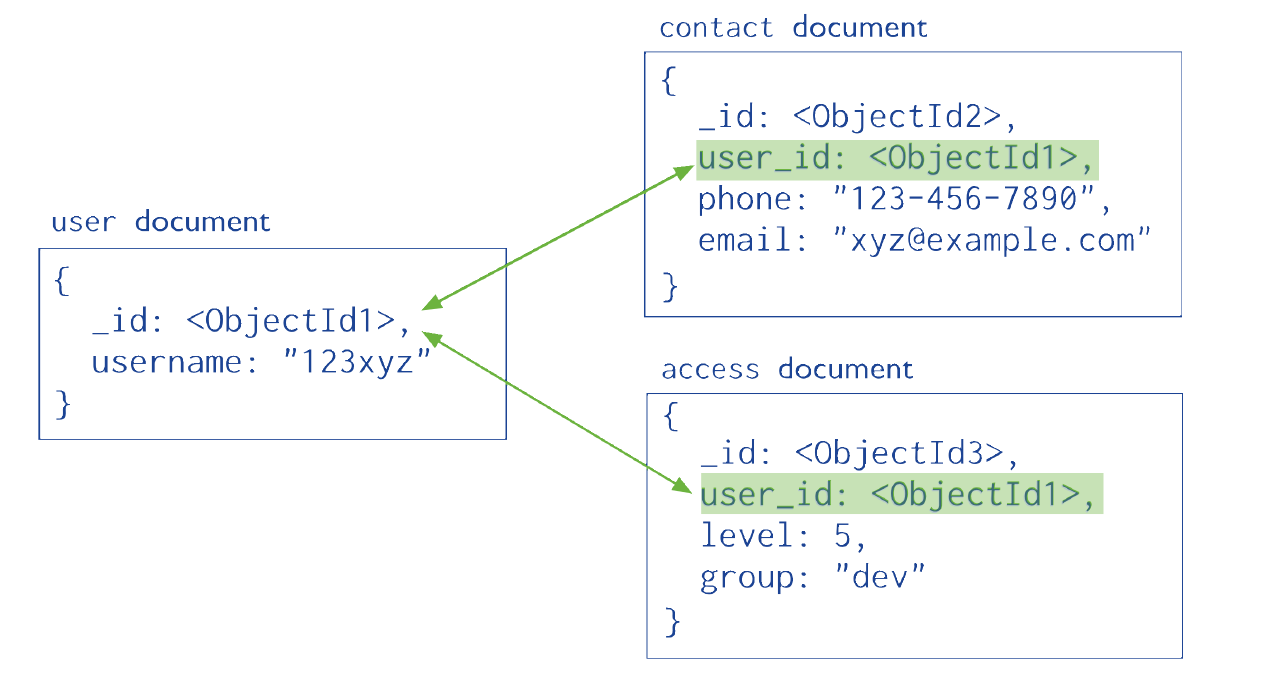
\includegraphics[width=.5\textwidth]{img/mongodb-reference}
		%{img/mongo/mongodb-reference}
		%\caption{R-tree structure}
		\label{fig:mongodb-ref-doc}
	}
	\centering
	\subfloat[Embedded document]{
		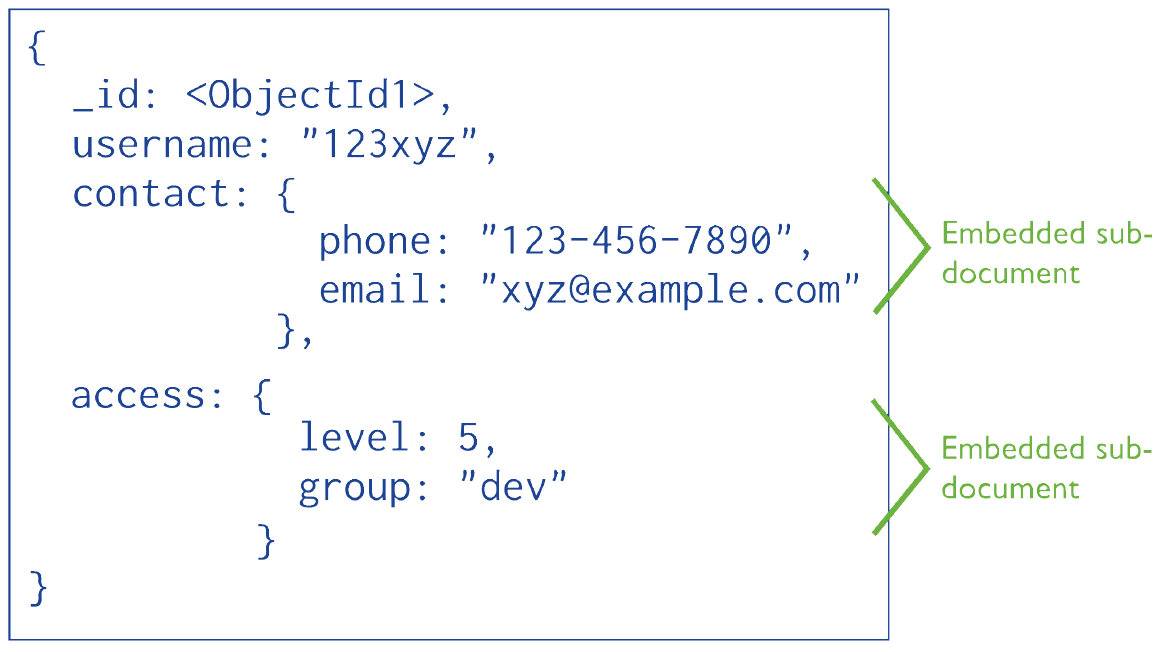
\includegraphics[width=.46\textwidth]{img/mongo/mongodb-embedded}
		%\caption{R-tree}
		\label{fig:mongodb-emb-doc}
	}
	\caption{MongoDB document structure~\citep{mongodb:org}}
	\label{fig:mongodb-doc}
	
\end{figure}

	\begin{figure}[h]
	\begin{lstlisting}[language=JSON,basicstyle=\scriptsize]
	{
		_id : "1"
		title : " MongoDB ",
		last_editor : "172.5.123.91" ,
		last_modified : new Date ("9/01/2015") ,
		body : " MongoDB is a..." ,
		categories : ["A", "B"] ,
		reviewed : false
	}
	\end{lstlisting} 
	\caption{MongoDB sample document}
	\label{sample-mongodb-document}
\end{figure}

\subsubsection{Indexing}\label{mong-xmark-indexing}

Each document in MongoDB is uniquely identified by a field \textit{\_id} which is also a primary index. Hence, the collection is sorted by \textit{\_id}~\citep{nosql/comparision}.
Apart from the primary index, MongoDB provides a mechanism to create secondary indexes for all fields of document. It supports various user defined indexes for field values including single field index, multikey index, multidimensional index, geo-spatial index, text index and hash index.
%Single field, multidimensional and multikey indexes are organized using B-tree, whereas geospatial index is implemented using quad trees.Once index is defined on a field,
\begin{itemize}
\item \textit{Single field index} only includes data from a single field of documents in a collection. 
\item \textit{Compound index} holds reference to the multiple fields within a collection's documents.
\item To index a field that contains an array value, MongoDB provides special indexing called \textit{Multikey index}.
\item \textit{Text index} helps efficient search of a string in documents.
\end{itemize}
\subsubsection{Query Model}\label{mongo-query-model}

%\todo{modify with christian's suggestions}
Queries in MongoDB are expressed in a JSON-like syntax and are sent to MongoDB as BSON objects by a database driver\citep{orend2010analysis}. A query can be specified by exact match on the embedded document or by using individual field with a \textit{dot notation}. It is used to access an element in document of an array or an object in the form of  $<$$array$.$index$$>$ or  $<$$object$.$childobject$$>$. For general queries, mongo shell can be used. It is an user friendly JavaScript shell that allows to implement callback functions to manipulate the data returned by the queries.  

\begin{comment}
\par
The Query model supports the following features:
\begin{enumerate}
	\item Queries over documents, embedded subdocuments and arrays
	\item Comparison operators
	\item Conditional Operators
	\item Logical Operators: AND and OR
	\item Sorting 
	\item Grouping
	\item Aggregation per query
\end{enumerate}
\end{comment}

The \textit{find()} method is the most common way to retrieve data from a collection. It returns the subset of documents from specified collection with given criteria that are passed as parameters. If no any parameters is given, it returns everything from a collection.  

\begin{comment}
The General syntax of find operation is given in Code~\ref{mongodb-find-sample}.
\begin{lstlisting}[language=JSON,caption=\textit{find} in MongoDB, label=mongodb-find-sample][H]
    db.collection.find(query, projection) 
\end{lstlisting}
 The \textit{query} specifies the criteria of document of a collection name \textit{collection}. The \textit{projection} selects of attributes of an documents to be return. For example, Code~\ref{mongodb-find-real} return the \textit{name} and \textit{age} from a collection  \textit{people} of country \textit{France} and \textit{age} is less than 5. 
\begin{lstlisting}[language=JSON,caption=\textit{find()} with query and project, label=mongodb-find-real][H]
    db.people.find({country:"France", age:{$lt:5}}, {_id:0, age:1, name:1}) 

\end{lstlisting}
\end{comment}

\par
\paragraph{Aggregation Frameworks:}
 The \textit{find} method is not sufficient for the complex database queries like aggregation, grouping  and advanced data manipulation. MongoDB provides two frameworks for advanced query as well as parallel processing for the large collection:
 \begin{description}
		\item[Aggregation pipeline]  \hfill \\
		The aggregation pipeline allows to execute series of operations using different operators like filtration, projection to produces desire result or performs aggregate operation.  It can be used for a single collection and uses  data operators like match, group, project, etc. in different stages. Every stage convert the documents as they pass through the pipeline. Data operators can be used  in any numbers of times.  The \textit{aggregate} function is responsible for this framework where it operates on a collection passing  entire documents into a pipeline. By using proper filtration operators like  skip, match and limit at the beginning  stage of the pipeline,  the frameworks can take advantages of existing indexes with processing scope limited to subset of documents, hence produces better performance in following stages~\cite{mongodbaggregation}. The aggregation pipeline has many limitations including data types, memory restriction to operators and output size~\cite{nosql/comparision}. 
		
\begin{comment}		
		Only 100 MB of RAM is assigned to pipeline stages. If this limit exceeds, the query will be broken. An option \textit{allowDiskUse} must be enable to write data to temporary files during staging.
		
				   \begin{lstlisting}[language=JSON,caption=An example Aggregation pipeline in MongoDB, label=mongodb-aggregation-pipeline, basicstyle = \scriptsize][h]
            db.open_auctions.aggregate([
                {$match:{reserve:{$exists:true}}},
		       {$project:{_id:0,reserve:{$multiply:["$reserve",2.20371]}}}
		       ]);
		  \end{lstlisting}
		  
\end{comment}
\item[MapReduce]  \hfill \\
		  The MapReduce is a data processing framework design to support large volumes of data that goes beyond the limitations and restriction of aggregation pipeline.  In mapreduce,  \textit{map} function applies to each input document and emits the key-value pair as output. Any arbitrary sorting and limiting  of single collection is performed before map stage. The reduce applies to the map's output where a key is associated with multiple values to return the aggregated data. The output of \textit{reduce} may pass optionally through finalize function to further process the result. Mapreduce functions are written in JavaScript and executed in MongoDB's demon process ~\cite{mongodbaggregation}.  Unlike pipeline framework, Map-reduce support options for choosing to store result  data in a node as collection or return the output.
\begin{comment}		  
		  Table~\ref{mongdb-mapreduce} illustrates a Mapreduce implementation in MongoDB. Two JavaScript function are defined for map and reduce. The \textit{runCommand} executes these functions in a collection.
		  
\end{description}		

\begin{longtable}{c|c}
\caption{Mapreduce in MongoDB}
 \label{mongdb-mapreduce}\\
	
	{\textit{map}} function(a) & {\textit{reduce}} function(b)\\
	\hline
	\begin{minipage}{.4\textwidth}
		\centering		
		\begin{lstlisting}[language=XML,basicstyle = \scriptsize,label=couchbase-map-sample]
map = function() {
           if(this.reserve){
            emit(this._id, this.reserve);
           }    
        };	
		\end{lstlisting}		
	\end{minipage} &
	\begin{minipage}{.49\textwidth}
		\centering
		\begin{lstlisting}[language=JSON, basicstyle =\scriptsize, label=couchbase-reduce-sample]
reduce = function(key,values) {
            return Array.sum(values);
        };
};
		\end{lstlisting}
	\end{minipage}
	\\
	\hline
	\multicolumn{2}{c}{
	    \scriptsize
	    
	Use: 	db.runCommand({"mapreduce" : 
	\textit{collectionName}, 
	                       "map" : \textit{map}, 
	                       "reduce" : \textit{reduce}})
		
	}
  	
  	\\
	\hline
	
\end{longtable}

\begin{end}	


\begin{comment}


\paragraph{System Architecture}
MongoDB can be run in two modes. In stand-alone mode, a single \textit{mongod} demon runs in a single node without any distribution and in shared mode various services are distributed to several nodes. 
\begin{figure}[h]
	\centering
	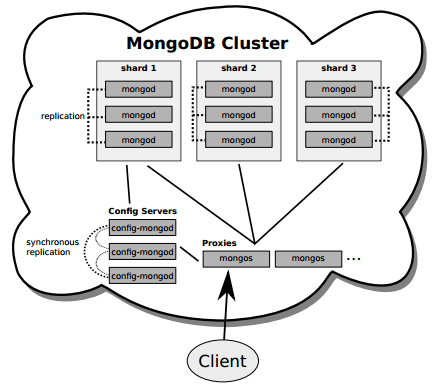
\includegraphics[width=0.5\textwidth]{img/mongo/clusters}
	%\caption{R-tree}
	\label{fig:mongodb-clusters}
\caption{MongoDB Clusters}
\end{figure} %reference




\end{comment}